\section{Experimental Results}
For initial improvements the transition parameters have been chosen since they are fewer than the states parameters. Due to time limitations, the initial search for best parameters is done by simple
iteration over arbitrary values for all parameters. An initial value is set and a delta parameter is added until it reaches the maximum value established.


\begin{table}[h]
\renewcommand{\arraystretch}{1.3}
\caption{Parameters Used for Enhancement}
\label{parameter_table}
\centering
\begin{tabular}{c||c||c||c}
\hline \bfseries $p$ &\bfseries $p_0$ &\bfseries $ p_{max}$ &\bfseries $\Delta p$ \\
\hline
\hline MSD & $20$ & $200$ & $5$ \\ 
\hline LE & $-1$ & $-0.8$ & $0.1$ \\ 
\hline RE & $0.8$ & $1$ & $0.1$ \\ 
\hline ST & $30$ & $300$ & $10$ \\ 
\hline 
\end{tabular} 
\end{table}

In the end 8658 combinations were generated and properly tested in \textit{CG Speedway 1} and \textit{B-Speedway}. The best result generated used the following parameters: MSD: $20$, LE: $-0.8$, RE: $1$, ST: $110$. This set of values generated the best result for \textit{B-Speedway} as well. An huge amount of parameters combination achieved the same best result in the second track. All of them do not trigger a state transition.



% apenas para GC, na B-speedway não tem alteração de estado

%  MAX\_SPEED\_DIST, the maximum distance for recognizing a curve.
%  LEFT\_EDGE, track position value that indicate the left boundary of the track.
%  RIGHT\_EDGE, track position value that indicate the right boundary of the track
%  STUCK\_TICKS, number of ticks required to leave the stuck state.
% }

% b-speedway,  tabs 1 e 2
% MAX\_SPEED\_DIST 70
%  LEFT\_EDGE, -1 (distancia proporcional do extremo da pista em relação ao meio)
%  RIGHT\_EDGE 1 (distancia proporcional do extremo da pista em relação ao meio)
%  STUCK\_TICKS 100

For each configuration, experiments consisted of 3 laps, in the B-Speedway and 
CG-Speedway 1 tracks (see Fig. \ref{fig:tracks}), each race starting with the car fully stopped. B-Speedway provides the simplest track for validation, while CG-Speedway 1
has more characteristics of usual race tracks, such as sharp curves for either side,
and provides a more general idea of the controller's behavior.

The total race time is being taken in account. A good set of parameters is the one that generates a low race time, the best set of parameters generated de lowest race time. Only time is being considerated at this time. Though damage and best lap time have significant impact in the final score.

The very first results emphasize this controller achievements: a better performance in more simple tracks, like oval ones, rather than in those with a higher degree of elaboration, like road or dirty tracks.


\begin{figure}[!t] 
\centering 
\subfloat[B-Speedway]{
\includegraphics[width=1.2in]{B-Speedway}}
% \label{fig_first_case}} 
\hfill
\subfloat[CG-Speedway]{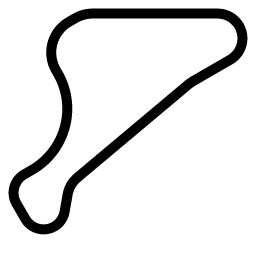
\includegraphics[width=1.2in]{CG-Speedway}}
% \label{fig_second_case}} 
\caption{FSMDriver test tracks.} 
\label{fig:tracks} 
\end{figure} 

When racing in oval tracks, particularly in B-Speedway, the FSMDriver outperforms 
some of the controllers provided by the TORCS distribution, specially that considered average drivers like Berniw 10. Pilots ran alone and total time was then reckoned (see Table \ref{table_results_B}).

For the sake of comparison the pilots provided by the TORCS distribution were used in those experiments. One of the best family of pilots is the Berniw set of drivers, which were chosen for comparison. \toDo{MELHORAR A FRASE}

\begin{table}[h]
\renewcommand{\arraystretch}{1.3}
\caption{Results After 3 Laps in B-Speedway}
\label{table_results_B}
\centering
\begin{tabular}{c||c||c||c}
\hline
\bfseries Driver & \bfseries Total Time & \bfseries Damage & \bfseries Top Speed \\ 
\hline
\hline Berniw 1 & 02:25:65 & 6 & 321 \\
\hline Berniw 2 & 02:25:65 & 6 & 321 \\
\hline Berniw 7 & 02:27:20 & 0 & 308 \\
\hline Berniw 6 & 02:27:46 & 0 & 309 \\
\hline Berniw 8 & 02:27:75 & 0 & 307 \\
\hline Berniw 9 & 02:28:10 & 0 & 306 \\
\hline Berniw 5 & 02:28:58 & 2 & 307 \\
\hline Berniw 4 & 02:29:42 & 3 & 303 \\
\hline Berniw 3 & 02:31:38 & 0 & 301 \\
\hline FSMDriver & 02:34:95 & 1 & 299 \\ 
\hline Berniw 10 & 02:40:70 & 8 & 282 \\ 
\hline 
\end{tabular}
\end{table}


Although, when it comes to road tracks, especially the ones filled with critical curves combinations, the controller faces several problems at staying between the track boundaries. These troubles are mainly caused by entering curves with high speed values, fact that reinforces the idea of an approaching curve state, to deal with speed reductions and angle corrections. The damage taken can be significantly reduced by implementing among with the approaching curve state, an enemy avoidance and overtaking behavior. In addition, the constants used in transition process do not represent the optimal values for that role, an evolutionary method needs to be implemented in order to achieve those values instead of the exhaustive search employed here. Moreover, oval tracks barely requires a state transition, in the overwhelming majority of time the car fits in the straight state. This lack of transitions and accentuated curves improves significantly the gain in performance.

\begin{table}[h]
\renewcommand{\arraystretch}{1.3}
\caption{Results After 3 Laps in CG Speedway 1}
\label{table_results_CG}
\centering

\begin{tabular}{c||c||c||c}
\hline \bfseries Driver &\bfseries Total Time &\bfseries Damage &\bfseries Top Speed \\
\hline
\hline Berniw 8 & 02:07:17 & 0 & 246 \\
\hline Berniw 6 & 02:07:18 & 0 & 248 \\
\hline Berniw 4 & 02:07:18 & 0 & 246 \\
\hline Berniw 7 & 02:07:20 & 0 & 250 \\
\hline Berniw 5 & 02:07:28 & 0 & 246 \\
\hline Berniw 3 & 02:07:28 & 0 & 247 \\
\hline Berniw 9 & 02:07:58 & 0 & 247 \\
\hline Berniw 1 & 02:12:80 & 1 & 252 \\
\hline Berniw 2 & 02:12:80 & 1 & 252 \\
\hline Berniw 10 & 02:21:54 & 0 & 230 \\
\hline FSMDriver & 02:34:49 & 3337 & 242 \\ 
\hline 
\end{tabular}
\end{table}
This approach demands a lot of time and space since all combinations are generated and executed. For future evolutions a more robust method, like genetic algorithm or neural networks needs to be applied in order to provide reliable results.
